\documentclass[a4paper,11pt]{article}
\usepackage[english]{babel}
\usepackage[T1]{fontenc}
\usepackage[latin1]{inputenc}
\usepackage[margin=34mm]{geometry}
\usepackage{pxfonts,charter}
\usepackage[expert]{mathdesign}
\usepackage[defaultsans]{opensans}
\usepackage{tabularx,longtable,booktabs,colortbl,multicol,listings,pdflscape}
\usepackage{color,graphicx,psfrag,float,subfig,pstool,ifpdf,dirtree,caption,enumitem}
\captionsetup{singlelinecheck=off}

\usepackage{zi4}
\usepackage{hyperref}
\makeatletter
\newcommand*{\centerfloat}{%
  \parindent \z@
  \leftskip \z@ \@plus 1fil \@minus \textwidth
  \rightskip\leftskip
  \parfillskip \z@skip}
\makeatother
\title{metabomatching}
\author{Rico Rueedi}
\date{February 15th, 2017}
\begin{document}
\maketitle\quad\\[16mm]
Updates on:
\begin{center}\href{http://www.unil.ch/cbg/index.php?title=metabomatching}{www.unil.ch/cbg/index.php?title=metabomatching}\end{center}
Please address any questions, comments, or bugs to
\begin{center}
\href{mailto:metabomatching@unil.ch}{metabomatching@unil.ch}
\end{center}
For bugs, please mention the version of metabomatching that produced the error. If possible, include the relevant \verb|ps.<description>| subdirectories.
\tableofcontents
\clearpage
\section{Quick Start}
\subsection{Docker}
The simplest method to run metabomatching is to use the metabomatching docker image. With a working \href{http://www.docker.com/products/overview}{docker} installation, run
\begin{verbatim}
  docker pull metabomatching/metabomatching-pre
\end{verbatim}
to download the metabomatching container. The download may take some time, as the container includes a full Linux operating system, octave to run metabomatching, and inkscape to convert metabomatching figures from SVG to PDF. 
\paragraph{Minimal Run} Run
\begin{verbatim}
  docker run -i -v <directory>:/mm-ps metabomatching/metabomatching-pre
\end{verbatim}
with \verb|<directory>| the absolute path to the local directory to which you want metabomatching to write its results. This runs metabomatching with default settings on a default pseudospectrum.

%To run metabomatching on data other than the included pseudospectrum data, all that is required is at least one pseudospectrum file named \texttt{<tag>.pseudospectrum.tsv} saved to a subdirectory named \texttt{ps.<description>} of \verb|<directory>|, and conforming to the format described in section \ref{sec:pseudospectra}.
\subsection{Matlab/octave}
The metabomatching Matlab code, which is compatible with octave, can be obtained from GitHub. The download includes: code files to run metabomatching and produce SVG images of the results, spectral reference databases built from HMDB and BMRB, a CASRN to metabolite name conversion list, and a test pseudospectrum.
\paragraph{Minimal Run} In Matlab/octave, set as working directory the directory into which metabomatching was downloaded, and run the file
\begin{verbatim}
   metabomatching.m
\end{verbatim}
This will apply metabomatching with default settings to the test pseudospectrum located in the subdirectory \verb|ps.test|. The metabomatching scores for each metabolite are stored in the 4th column of the tab-separated file \verb|ps.text/test.scores.tsv| and presented graphically in the file \verb|ps.test/test.svg|.
%To run metabomatching on data other than the provided test data, all that is required is at least one pseudospectrum file named \texttt{<tag>.pseudospectrum.tsv} saved to a subdirectory named \texttt{ps.<description>}, and conforming to the format described in section \ref{sec:pseudospectra}.
\clearpage
\section{Complete Instructions}
Metabomatching operates on the contents of the directory in which it is installed. Specifically, for each subdirectory of the installation directory named \begin{verbatim}
   ps.<description>
\end{verbatim}
metabomatching will be run over all pseudospectrum files named
\begin{verbatim}
   <tag>.pseudospectrum.tsv
\end{verbatim}
within. Metabomatching settings are fixed for each subdirectory, and all pseudospectra within a subdirectory must be defined on the same chemical shift binning. Details on the content and format of pseudospectra files are given in section \ref{sec:pseudospectra}.

\paragraph{Example.} Suppose we would like to apply metabomatching to the pseudospectra of two SNPs, rs1 and rs2, obtained in one association study (study1), and to the pseudospectra of two SNPs, rs1 and rs3, obtained in another study (study2). Using the SNP names as tags for the pseudospectra and the study names as description for the subdirectories, the folder structure in the installation should then be
\begin{verbatim}
   <installation directory>/
   |-- data/
       |-- ...
   |-- documentation/
       |-- ...
   |-- fos/
       |-- ...
   |-- func/
       |-- ...
   |-- ps.study1/
   |   |-- rs1.pseudospectrum.tsv
   |   |-- rs2.pseudospectrum.tsv
   |-- ps.study2/
   |   |-- rs1.pseudospectrum.tsv
   |   |-- rs3.pseudospectrum.tsv
   |-- metabomatching.m
\end{verbatim}
\paragraph{Metabomatching Results.} For each pseudospectrum file
\begin{verbatim}
   <tag>.pseudospectrum.tsv
\end{verbatim}
in each subdirectory, metabomatching outputs one scores file 
\begin{verbatim}
   <tag>.scores.tsv
\end{verbatim}
and one SVG file
\begin{verbatim}
   <tag>.svg
\end{verbatim}
showing the main metabomatching results. If running the metabomatching docker the SVG file is also converted to PDF, resulting in the additional PDF file
\begin{verbatim}
   <tag>.pdf
\end{verbatim}
 Details on the content and format of scores files are given in section \ref{sec:pseudospectra}. Details for the SVG/PDF files are given in section \ref{sec:svg}. For each subdirectory, metabomatching also writes files related to the settings and reference data used. These are described in section \ref{sec:settings}.
\paragraph{Spectral Reference Data.} Metabomatching compares pseudospectra to NMR spectra listed in a reference database. The \verb|data| subdirectory in the installation directory contains nine databases. Six contain reference spectra from HMDB, three from BMRB. Details as to their content and format are given in section \ref{sec:databases}.
\subsection{Pseudospectra and Scores\label{sec:pseudospectra}}
For an untargeted metabolome composed of $N$ features, the pseudospectrum of a certain variable is the collection of $N$ association $p$-values, $N$ effect sizes, and $N$ standard errors resulting from the associations of the variable with the $N$ metabolome features.
\subsubsection{Pseudospectrum file format, one per file.} A pseudospectrum is provided to metabomatching as a tab-separated file named 
\begin{verbatim}
   <tag>.pseudospectrum.tsv
\end{verbatim}
The file contains four columns. The first row must be a header line containing the four labels \verb|shift|, \verb|beta| (effect size), \verb|se| (standard error), and \verb|p|. The subsequent $N$ rows contain the association data for the $N$ metabolome features, indexed by their chemical shift. Columns and data rows may appear in any order. The tag may be composed of letters, numbers, hyphens, and underscores.
\paragraph{Example.} Pseudospectrum file with the header row and three data rows.
\begin{verbatim}
   shift   beta    se      p
   1.11    0.03041 0.08991 0.2647  
   1.12    -0.5301 0.8771  6.1451E-11
   1.13    -0.7171 0.1871  0.003201
\end{verbatim}
\paragraph{Scores file format.} For every pseudospectrum, metabomatching computes $M$ scores, with $M$ the number of metabolite reference spectra provided, and writes the corresponding scores file, named 
\begin{verbatim}
   <tag>.scores.tsv
\end{verbatim}
The file contains three columns, listing the metabolite CASRN, a spectrum identification number (see \ref{sec:databases}), and the metabomatching score.
\paragraph{Example.} Scores file for three metabolites.
\begin{verbatim}
   70-47-3 10003021     3.8131
   56-84-8 10003111     0.0002
   56-88-2 10003311     0.0002
\end{verbatim}
\subsubsection{Pseudospectrum file format, multiple per file.}
Multiple pseudospectra can be provided to metabomatching in a single tab-separated file, named
\begin{verbatim}
   <study_tag>.pseudospectrum.tsv
\end{verbatim}
For $K$ pseudospectra, the file contains $1+3K$ colums. The first row must be a header line containing the label \verb|shift|, and the set of labels \verb|beta/<tag>| (effect size), \verb|se/<tag>| (standard error), and \verb|p/<tag>| for each of the $K$ pseudospectra.
\paragraph{Example.} Pseudospectrum file with the header row and three data rows, for two pseudospectra, labeled \verb|rs18| and \verb|ex27|
\begin{verbatim}
   shift   beta/rs18      se/rs189 p/rs189 beta/ex72  se/ex27    p/ex27
   1.11    0.109   0.0871  0.207   0.556   0.0964  1.15E-08
   1.12    -2.66E-06       0.0872  0.999   -0.0154 0.0979  0.874
   1.13    -0.0634 0.0871  0.466   0.491   0.0964  4.37E-07
\end{verbatim}
\paragraph{Scores file format.} For every pseudospectrum, metabomatching computes $M$ scores, with $M$ the number of metabolite reference spectra provided, and writes the corresponding scores file, named 
\begin{verbatim}
   <study_tag>.scores.tsv
\end{verbatim}
The file contains $2+K$ columns, listing the metabolite CASRN, a spectrum identification number (see \ref{sec:databases}), and the metabomatching score for each of the $K$ pseudospectra.
\paragraph{Example.} Scores file for three metabolites and two pseudospectra labeled \verb|rs189| and \verb|ex27|
\begin{verbatim}
   cas     id      score/rs189     score/ex27
   70-47-3 10003021        3.81    0.715
   56-84-8 10003111        0.002   1.21
   56-88-2 10003311        0.002   267
\end{verbatim}
\subsection{Settings\label{sec:settings}}
The settings used by metabomatching in each subdirectory can be specified with the optional file
\begin{verbatim}
   parameters.in.tsv
\end{verbatim}
There are seven settings that control the metabomatching algorithm, and two common graphical settings described below. Additional graphical settings are described in section \ref{sec:svg}. For any non-specified setting, metabomatching uses a default value. On completion, metabomatching writes all settings it used to the file
\begin{verbatim}
   parameters.out.tsv
\end{verbatim}
independently of whether the settings were provided or used by default.
\begin{table}[h]
\small
\centerfloat
\begin{tabularx}{1.2\linewidth}{@{}lXll@{}}
key & description & values & default \\
\midrule
\texttt{variant} & %
Select among the 1-compound, 2-compound, $\pm$-, and $\pm$-2-compound-variants of metabomatching. Note that 2-compound and $\pm$-2-compound metabomatching are computationally demanding, and may exceed the capabilities of standard personal computers.& %
\begin{tabular}[t]{@{}ll@{}}\texttt{1c}&\texttt{2c}\\\texttt{pm}&\texttt{pm2c}\end{tabular}&\texttt{1c}\\
\texttt{mode} & Controls the spectrum description type used by metabomatching, and determines, in conjunction with setting \texttt{reference}, the spectral reference file metabomatching tries to load. & %
\begin{tabular}[t]{@{}l@{}}\texttt{peak}\\\texttt{multiplet}\end{tabular} & %
\texttt{peak} \\
\texttt{dsh} & %
Controls the neighborhood parameter ($\delta$ if in peak mode, $\gamma$ if in multiplet mode). & %
$(0,1]$ & %
\begin{tabular}[t]{@{}l@{}}$0.025$ ($\delta$)\\ $0.01$ ($\gamma$)\end{tabular}\\
\texttt{scoring} & Selects the type of scoring used in the match sum & \texttt{chisq z} & \texttt{chisq} \\
\texttt{decorr\_lambda} & Sets the shrinkage parameter $\lambda$ used when applying decorrelation. $\lambda=1$ implies no decorrelation. & $[0,1]$ & 1\\
\texttt{p\_pm} & Sets the $p$-value threshold below which pseudospectrum features are considered to carry signal (rather than noise) for the purpose of $\pm$-metabomatching (\texttt{variant = pm} or \texttt{pm2c}). When running metabomatching for one effect direction, the effect size for features of association $p$-value below \texttt{p\_suggestive} and of opposite effect direction is set to 0. & $[0,0.05]$ & \texttt{1E-4}\\
\texttt{reference} & %
Selects which of the four standard reference sets metabomatching uses. Metabomatching copies the corresponding reference file to each subdirectory. Metabomatching uses the specified reference set in combination with any \verb+slo(m|p)+ files already present in the subdirectory. If \verb|reference| is set to \verb|existing|, metabomatching uses only reference file(s) already present in the subdirectory. This applies to both \verb+slo(m|p)+ files and \verb|casname| files. & %
\begin{tabular}[t]{@{}ll@{}}\texttt{hmdb}&\texttt{bmrb}\\\texttt{umdb}&\texttt{umrb}\\\texttt{smdb}&\texttt{smrb}\end{tabular} & %
\texttt{hmdb}\\
\texttt{n\_show} & %
Sets the number of candidate metabolites shown in the results SVG file. Due to the graphical layout, only multiples of 4 are allowed as values for \texttt{n\_show}. & %
4, 8, 12, \ldots &
8 \\
\texttt{p\_significant} & %
Sets the $p$-value threshold below which pseudospectrum features are considered significant. This has no effect on metabomatching, and serves only to label features in the SVG file. Significant features are clustered (distance below $2\delta$ if \texttt{mode = peak} or $2\gamma+0.3$ if \texttt{mode = multiplet}). High values for \texttt{p\_significant} may tag many features significant and break the layout of the SVG file. & %
$(0,0.05]$ & %
\texttt{5E-8} \\
\bottomrule
\end{tabularx}
\end{table}
For any other value in $[0,1)$ the feature-feature correlation matrix must be available in the subdirectory, as a comma-separated file named
\begin{verbatim}
   correlation.csv
\end{verbatim}
The file has no header or row descriptors, and should contain $N$ columns and $N$ rows, with $N$ the number of non header rows in the pseudospectra.
\subsection{Reference Spectral Databases\label{sec:databases}}
The spectral reference databases included with the metabomatching software were obtained from HMDB (Human Metabolome Database, DS Wishart et al., \emph{Nucleic Acids Res.}, 41:D801-7) and BMRB (Biomagnetic Resonance Database, EL Ulrich et al., \emph{Nucleic Acids Res.}, 36:D402-8). Resulting from different experiments, the spectra for individual metabolites are usually different in the two databases, sometimes significantly so.
\subsubsection{HMDB}
In HMDB, the spectrum for a metabolite is characterized twice. Once as a list of multiplets, and once as a list of peaks. For most spectra, the two descriptions are different enough to result in differences in metabomatching rankings. The differences can be significant. HMDB contains a proton NMR spectrum for 835 metabolites. Every metabolite in the database is identified by a metabolite ID of the form \verb|HMDB00001|.
\paragraph{Peak Descriptions File.} The full set of peak description metabolite spectra is listed in the reference file
\begin{verbatim}
   hmdb.slop
\end{verbatim}
This file is a four column tab-separated file, with each row containing the CASRN (as a string), the peak position in ppm (real number), the peak height (real number), and the spectrum ID (integer), for one peak of the peak description spectrum of one metabolite. The spectrum ID is defined as \verb|1<xxxxxx>1|, with \verb|<xxxxxx>| the HMDB ID stripped of the characters \verb|HMDB| but keeping leading zeroes. Peak heights are used in the SVG image, but not by metabomatching.
\paragraph{Example.} Spectra of dimethylglycine (CASRN 1118-68-9, HMDB00092) and glycine (CASRN 56-40-6, HMDB000123)
\begin{verbatim}
   1118-68-9   2.91    1.000   1000921
   1118-68-9   3.71    0.277   1000921
   56-40-6     3.54    1.000   1001231
\end{verbatim}

\paragraph{Multiplet Descriptions File.} The full set of multiplet description metabolite spectra is listed in the reference file
\begin{verbatim}
   hmdb.slom
\end{verbatim}
This file is a four column tab-separated file, with each row containing the CASRN (as a string), the left edge of the multiplet range (real number),  the right edge of the multiplet range (real number), the proton count (integer), and the spectrum ID (integer), for one multiplet range of the multiplet description spectrum of one metabolite. The spectrum ID is defined as \verb|1<xxxxxx>1|, with \verb|<xxxxxx>| the HMDB ID stripped of the characters \verb|HMDB| but keeping leading zeroes. Proton counts are used in the SVG image, but not by metabomatching.
\paragraph{Example.} Spectra of dimethylglycine (CASRN 1118-68-9, HMDB00092) and glycine (CASRN 56-40-6, HMDB000123)
\begin{verbatim}
   1118-68-9   2.90    2.93    6   1000921
   1118-68-9   3.70    3.72    2   1000921
   56-40-6     3.46    3.60    2   1001231
\end{verbatim}
\paragraph{Subsets.} Two additional reference files are available containing the spectra of metabolites known to be contained in urine samples. This subset was defined by Bouatra et al. (\emph{PLOS One}, 8(9):e73076), and named UMDB (Urine Metabolome Database). It lists the spectra for 180 metabolites. The files are named
\begin{verbatim}
   umdb.slop
   umdb.slom
\end{verbatim}
for the peak and multiplet description spectra, respectively. Similarly, two additional reference files are available containing the spectra of metabolites known to be contained in serum samples. This subset was defined by Gowda et al. (\emph{Anal. Chem.}, 86(11):5433-5440). It lists the spectra for 180 metabolites. The files are named
\begin{verbatim}
   smdb.slop
   smdb.slom
\end{verbatim}
\subsubsection{BMRB}
In BMRB, the spectrum for a metabolite is characterized as a list of peaks. Each metabolite can have several spectra, obtained from different experiments. For most spectra, the descriptions are different enough to affect, slightly, metabomatching rankings. BMRB contains 975 proton NMR spectra for 740 metabolites. Every metabolite in the database is identified by a metabolite ID of the form BMRB00001.
\paragraph{Peak Descriptions File.} The full set of peak description metabolite spectra is listed in the reference file
\begin{verbatim}
   bmrb.slop
\end{verbatim}
This file is a four column tab-separated file, with each row containing the CASRN (as a string), the peak position in ppm (real number), the peak height (real number), and the spectrum ID (integer) for one peak of the peak description spectrum of one metabolite. The spectrum ID is defined as \verb|2<xxxxxx><y>|, with \verb|<xxxxxx>| the BMRB ID stripped of the characters \verb|BMRB| but keeping leading zeroes, and \verb|<y>| indexes different spectra for the same BMRB metabolite. Peak height is used in the SVG image, but not by metabomatching.
\paragraph{Example.} Spectra of dimethylglycine (CASRN 1118-68-9, BMRB02411) and glycine (CASRN 56-40-6). Glycine appears in BMRB with two different BMRB IDs (BMRB00089 and BMRB00977), and has four listed spectra (3 for BMRB00089, and 1 for BMRB00977).
\begin{verbatim}
   1118-68-9   2.916   1.000   2002411
   1118-68-9   3.714   0.336   2002411
   56-40-6     3.541   1.000   2000891
   56-40-6     3.542   1.000   2000892   
   56-40-6     3.544   1.000   2000893
   56-40-6     3.545   1.000   2009771
\end{verbatim}
\paragraph{Subsets.} An additional reference file is available containing the spectra of metabolites known to be contained in urine samples. It lists the spectra for 180 metabolites. The file is named
\begin{verbatim}
   umrb.slop
   umrb.slom
\end{verbatim}
for the peak and multiplet description spectra, respectively. Similarly, an additional reference file is available containing the spectra of metabolites known to be contained in serum samples. It lists the spectra for 180 metabolites. The file is named
\begin{verbatim}
   smrb.slop
\end{verbatim}
\subsubsection{BMRB}
In BMRB, the spectrum for a metabolite is characterized as a list of peaks. Each metabolite can have several spectra, obtained from different experiments. For most spectra, the descriptions are different enough to affect, slightly, metabomatching rankings. BMRB contains 975 proton NMR spectra for 740 metabolites. Every metabolite in the database is identified by a metabolite ID of the form BMRB00001.
\subsubsection{Chemical Abstracts Service Registry Number (CASRN)}
Metabomatching uses CASRN (Chemical Abstracts Service Registry Number) to identify metabolites. Metabolite names are used only in the SVG image. The file
\begin{verbatim}
   all.casname
\end{verbatim}
provides the CASRN to metabolite name table, as a two column tab-separated file.
\paragraph{Example.} Entries for dimethylglycine and glycine
\begin{verbatim}
   1118-68-9   dimethylglycine
   56-40-6     glycine
\end{verbatim}
\subsubsection{Providing a Custom Spectral Reference Database}
Additional spectra can be provided to metabomatching as a custom spectral reference database. The database itself needs a name and a number (3 and above, as 1 and 2 are already assigned to HMDB and BMRB respectively). Each spectrum in the database needs a CASRN identifying the metabolite, and a 6 digit ID number indexing the metabolite in the database as well as a 1 digit number indexing different spectra for the same metabolite. 
\paragraph{Example.} To provide two new spectra for glycine and two new spectra for the new metabolite \emph{customine} in a custom database called MYDB, we would create the database file
\begin{verbatim}
   mydb.slop
\end{verbatim}
of content
\begin{verbatim}
   56-40-6     3.541   1.000   4000011
   56-40-6     3.542   1.000   4000012   
   12345-67-8  1.234   1.000   4000021
   12345-67-8  1.236   1.000   4000022   
\end{verbatim}
Because customine is not known in \verb|all.casname|, we would also create the CASRN-name table
\begin{verbatim}
   mydb.casname
\end{verbatim}
of content
\begin{verbatim}
   12345-67-8  customine
\end{verbatim}
Both \verb|mydb.slop| and \verb|mydb.casname| need to be placed in the \verb|ps.<description>| subdirectories for which metabomatching should use MYDB, and can be used exclusively, or in combination with a standard database (see \verb|reference| setting).
\section{Metabomatching Figures\label{sec:svg}}
For every \verb|<tag>.pseudospectrum.tsv| file in every \verb|ps.<description>| subdirectory, metabomatching creates an SVG image that shows the pseudospectrum and the spectra of the \verb|n_show| top-ranked candidate metabolites. The image is designed with a width of 180mm. It is optimized for use with the \texttt{Open Sans} font, freely available from \href{https://fonts.google.com/specimen/Open+Sans}{fonts.google.com}.

The SVG image for the test pseudospectrum included in the metabomatching download is shown in \ref{fig:1}. The SVG image for 2-compound metabomatching (\ref{fig:2}) has some slight differences.
\begin{figure}
\captionsetup{singlelinecheck=off}
\centerfloat
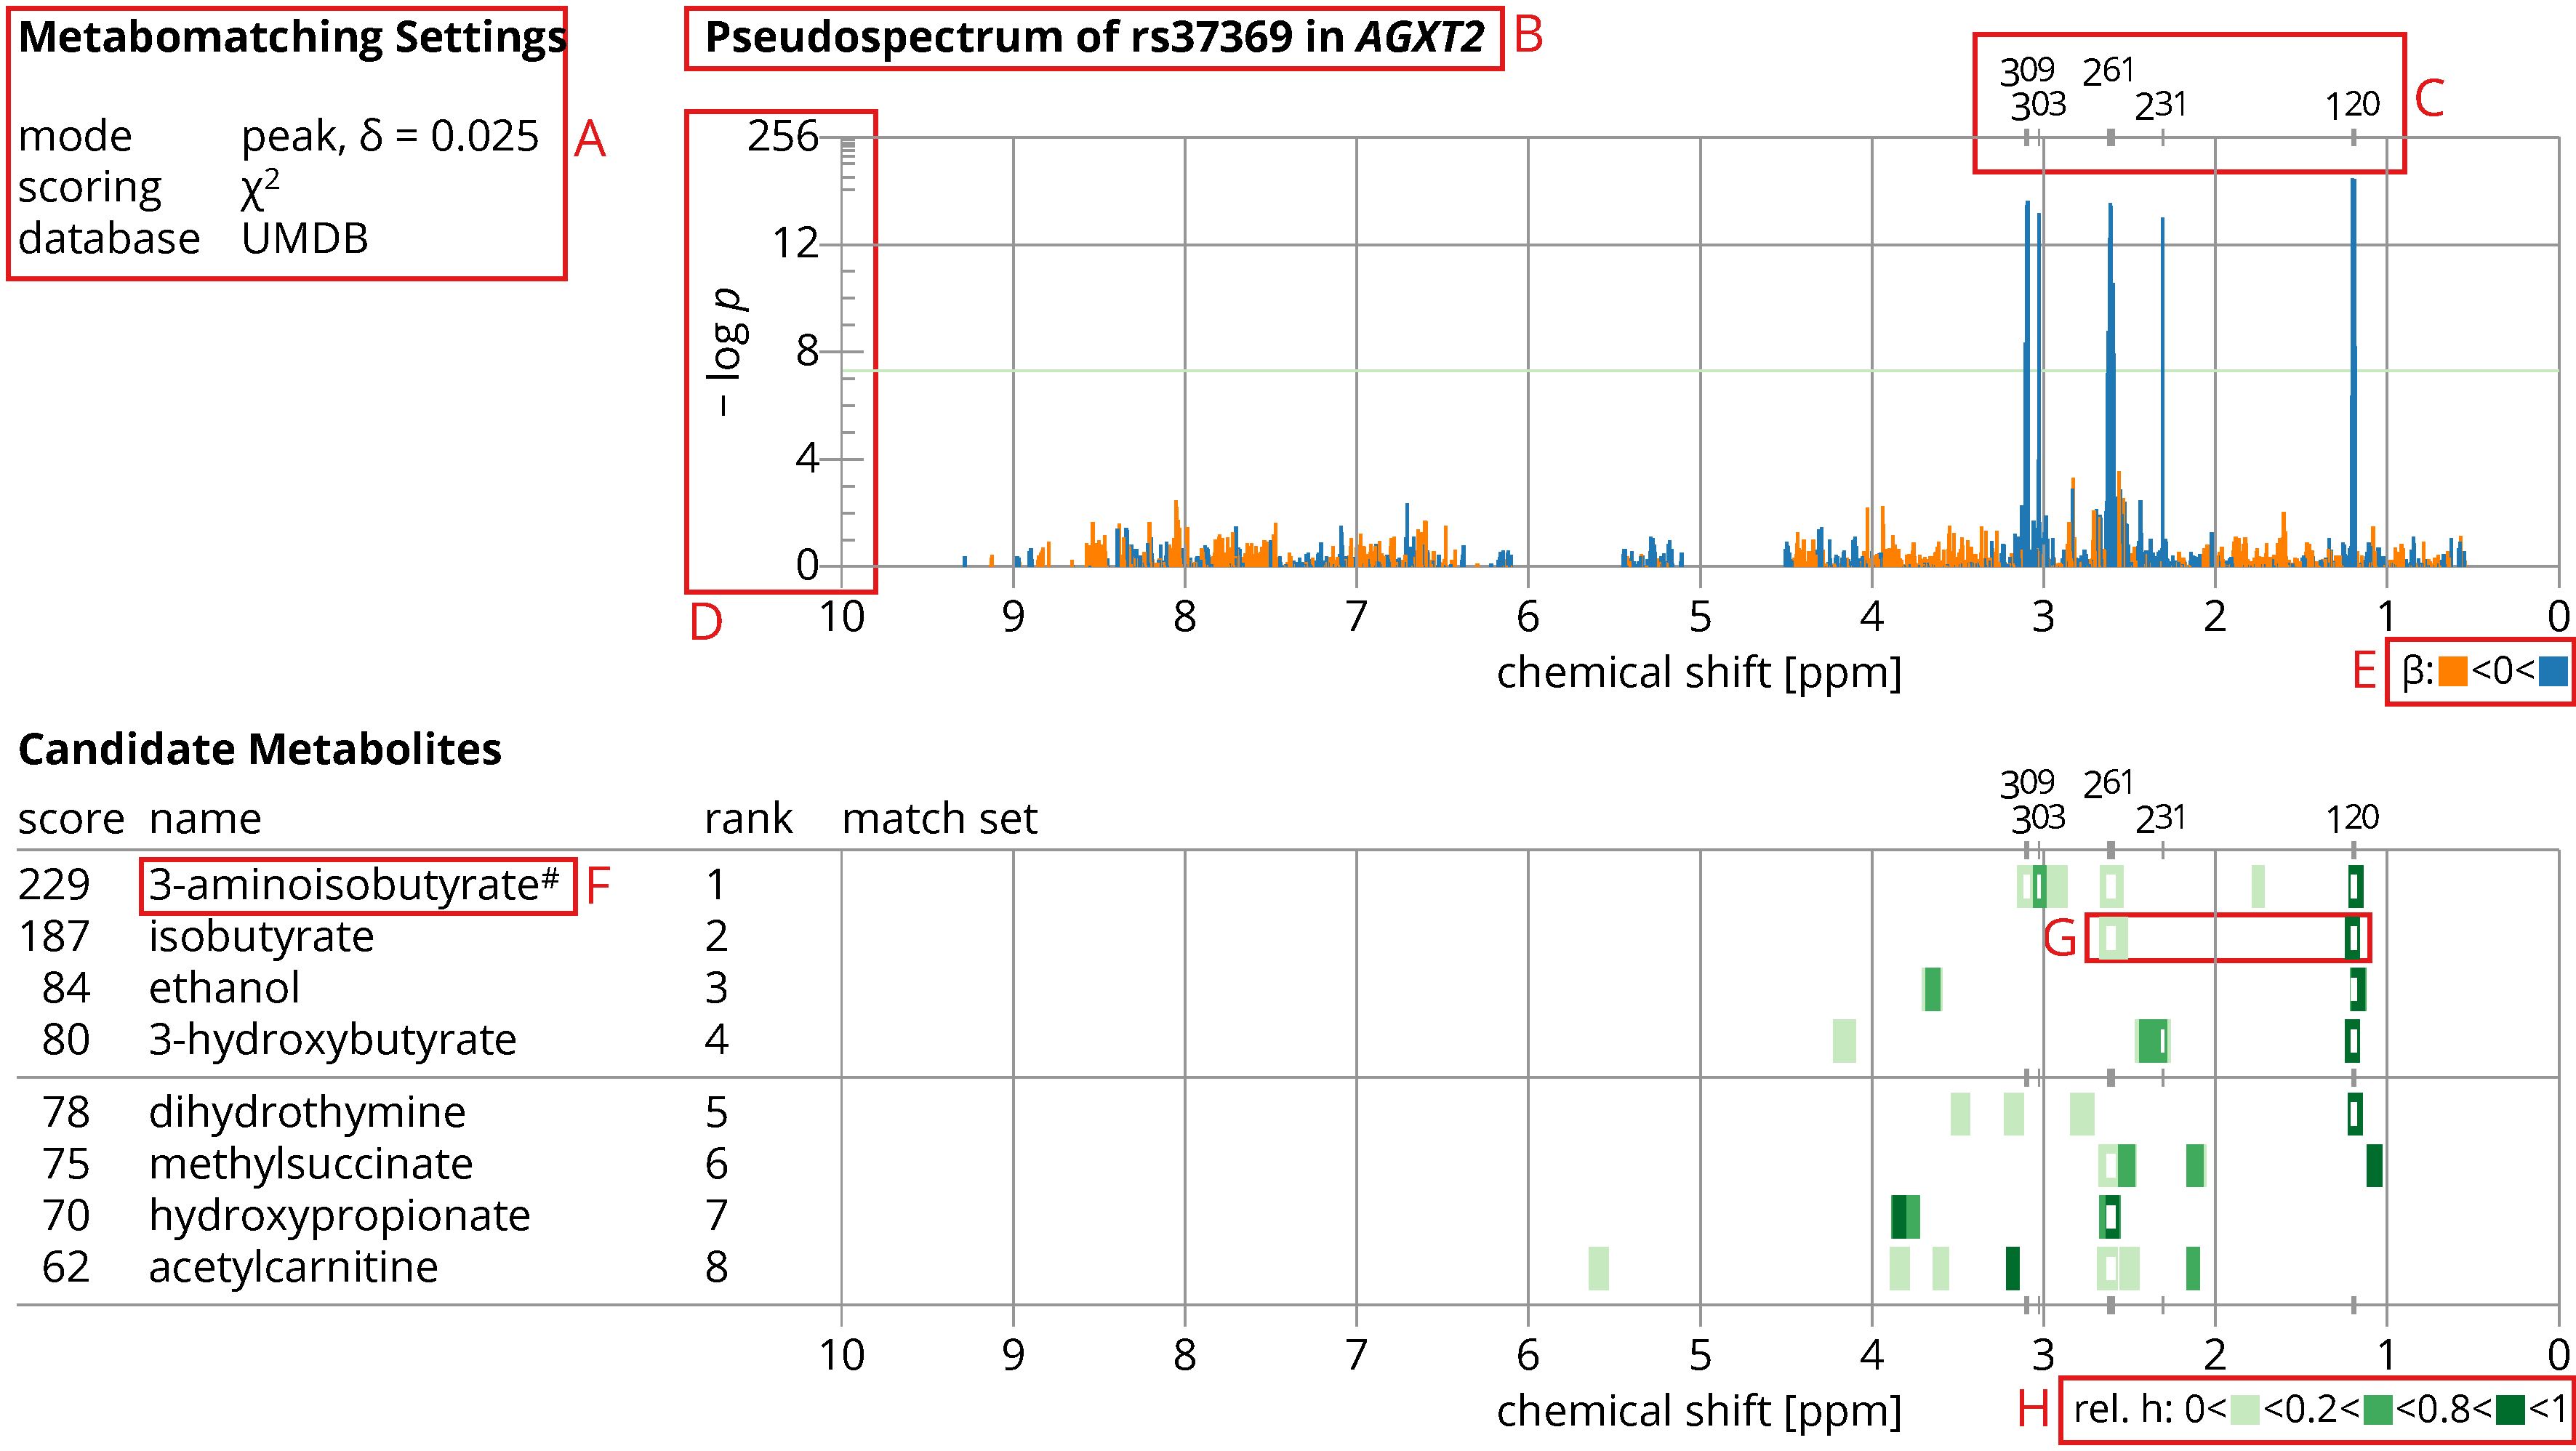
\includegraphics[width=180mm]{f1.pdf}
\caption[bla]{\label{fig:1}Metabomatching results for the pseudospectrum of SNP rs37369 in \emph{AGXT2}. The figure contains three panels: the settings panel (\emph{Metabomatching Settings}, top left), the pseudospectrum panel (\emph{Pseudospectrum of \ldots}, top right), and the spectrum panel (\emph{Candidate Metabolites}, bottom). %
\begin{description}[align=left,noitemsep,labelwidth=7.2mm]
\item[A.] The settings panel lists the main settings used in the metabomatching run. 
\item[B.] The title of the pseudospectrum panel can be provided by the user (see below).
\item[C.] Features in the pseudospectrum with $p$-value below the significance threshold defined by \texttt{p\_significant} are highlighted. The position of each significant feature is marked by a tick on the upper edge of the pseudospectrum box. In addition, significant peaks are clustered (according to $\delta$ or $\gamma+0.015$), and the position of the peak with the strongest association in the cluster is labeled. Marks are repeated in the spectrum panel.
\item[D.] The scale used for the pseudospectrum $y$-axis is linear for values of $-\log p$ between 0 and 12, logarithmic for values above 12, and capped at 256.
\item[E.] Features are colored orange if their association effect size $\beta$ is negative,  blue if it is positive.
\item[F.] A list of metabolites that are shown regardless of their ranks, can be provided by the user (see below). Such metabolites are marked by a "\#" next to their name.
\item[G, H.] The match sets are shown on the same chemical shift axis as the pseudospectrum, with one match set per row. For each match set element, the relative height of the peak that produced the element is color-coded. Elements are plotted in order of increasing relative height. In multiplet mode, relative proton counts are used instead of relative heights. The positions of significantly associated features are marked by white ticks in the match set rows to highlight match set elements that include these features.
\end{description} %
}
\end{figure}
\paragraph{Titles.} The titles for the metabomatching figures are provided  either with an additional \verb|description.tsv| file, or directly in the \verb|parameters.in.tsv| file.
\paragraph{} The \verb|description.tsv| file is a two-column tab-separated file, in which the first column contains the pseudospectrum tag and the second a description. The pseudospectrum panel title will then read
\begin{verbatim}
   Pseudospectrum of <description>
\end{verbatim}
in bold face. In the case where pseudospectra result from an mGWAS, the description file may be formatted as a three-column file, in which the first column contains the pseudospectrum tag, the second the SNP ID, and the third the gene name. The title will then read
\begin{verbatim}
   Pseudospectrum of <SNPID> in <GENE>
\end{verbatim}
in bold face and with the gene name in italics.
\paragraph{Example.} For the test pseudospectrum, the description file reads
\begin{verbatim}
   test    rs37369 AGXT2
\end{verbatim}
\paragraph{} In the \verb|parameters.in.tsv| file, descriptions are provided as
\begin{verbatim}
   description_<tag> <description>
\end{verbatim}
\paragraph{Control Metabolites.} Control metabolites are provided to metabomatching either with an additional \verb|cascontrol.tsv| file, or directly in the \verb|parameters.in.tsv| file.
\paragraph{} The \verb|cascontrol.tsv| file is a two column tab-separated file, in which the first column contains the tag of the pseudospectrum and the second the CASRN of the desired control metabolite. More than one control metabolite may be provided for any pseudospectrum, each in a new line.
\paragraph{Example.} For the test pseudospectrum, the \verb|cascontrol.csv| file reads
\begin{verbatim}
   test    144-90-1
\end{verbatim}
\paragraph{} In the \verb|parameters.in.tsv|, control metabolites are provided as
\begin{verbatim}
   cas_control_<tag>_<#>   <CASRN>
\end{verbatim}

%\subsection{Additional Graphical Settings}
%\subsubsection{ \texttt{ls}}
%Set metabomatching to produce 220mm wide figures suitable for landscape paper orientation (see figure \ref{fig:2}). In this orientation and space permitting, metabolite names are shown, but CASRN aren't. In 2-compound metabomatching, long metabolite names are replaced by metabolite CASRN. This option is applied, for all pseudospectra, by adding
%\begin{verbatim}
%   ls        1
%\end{verbatim}
%in the \verb|parameters.in.tsv| file.
%\subsubsection{ \texttt{title}}
%Adding
%\begin{verbatim}
%   title     0
%\end{verbatim}
%to the \verb|parameters.in.tsv| file sets metabomatching to not print the figure title (A) when in portrait orientation. The option has no effect in landscape mode.
%\subsubsection{\texttt{psa\_<tag>}}
%For cases where the labels for significant features (C) overlap the pseudospectrum title (B), the pseudospectrum title can be aligned to the right edge of the pseudospectrum panel. This is done for each pseudospectrum individually, by adding
%\begin{verbatim}
%   psa_<tag> right
%\end{verbatim}
%in the \verb|parameters.in.tsv| file.
\begin{figure}
\centerfloat
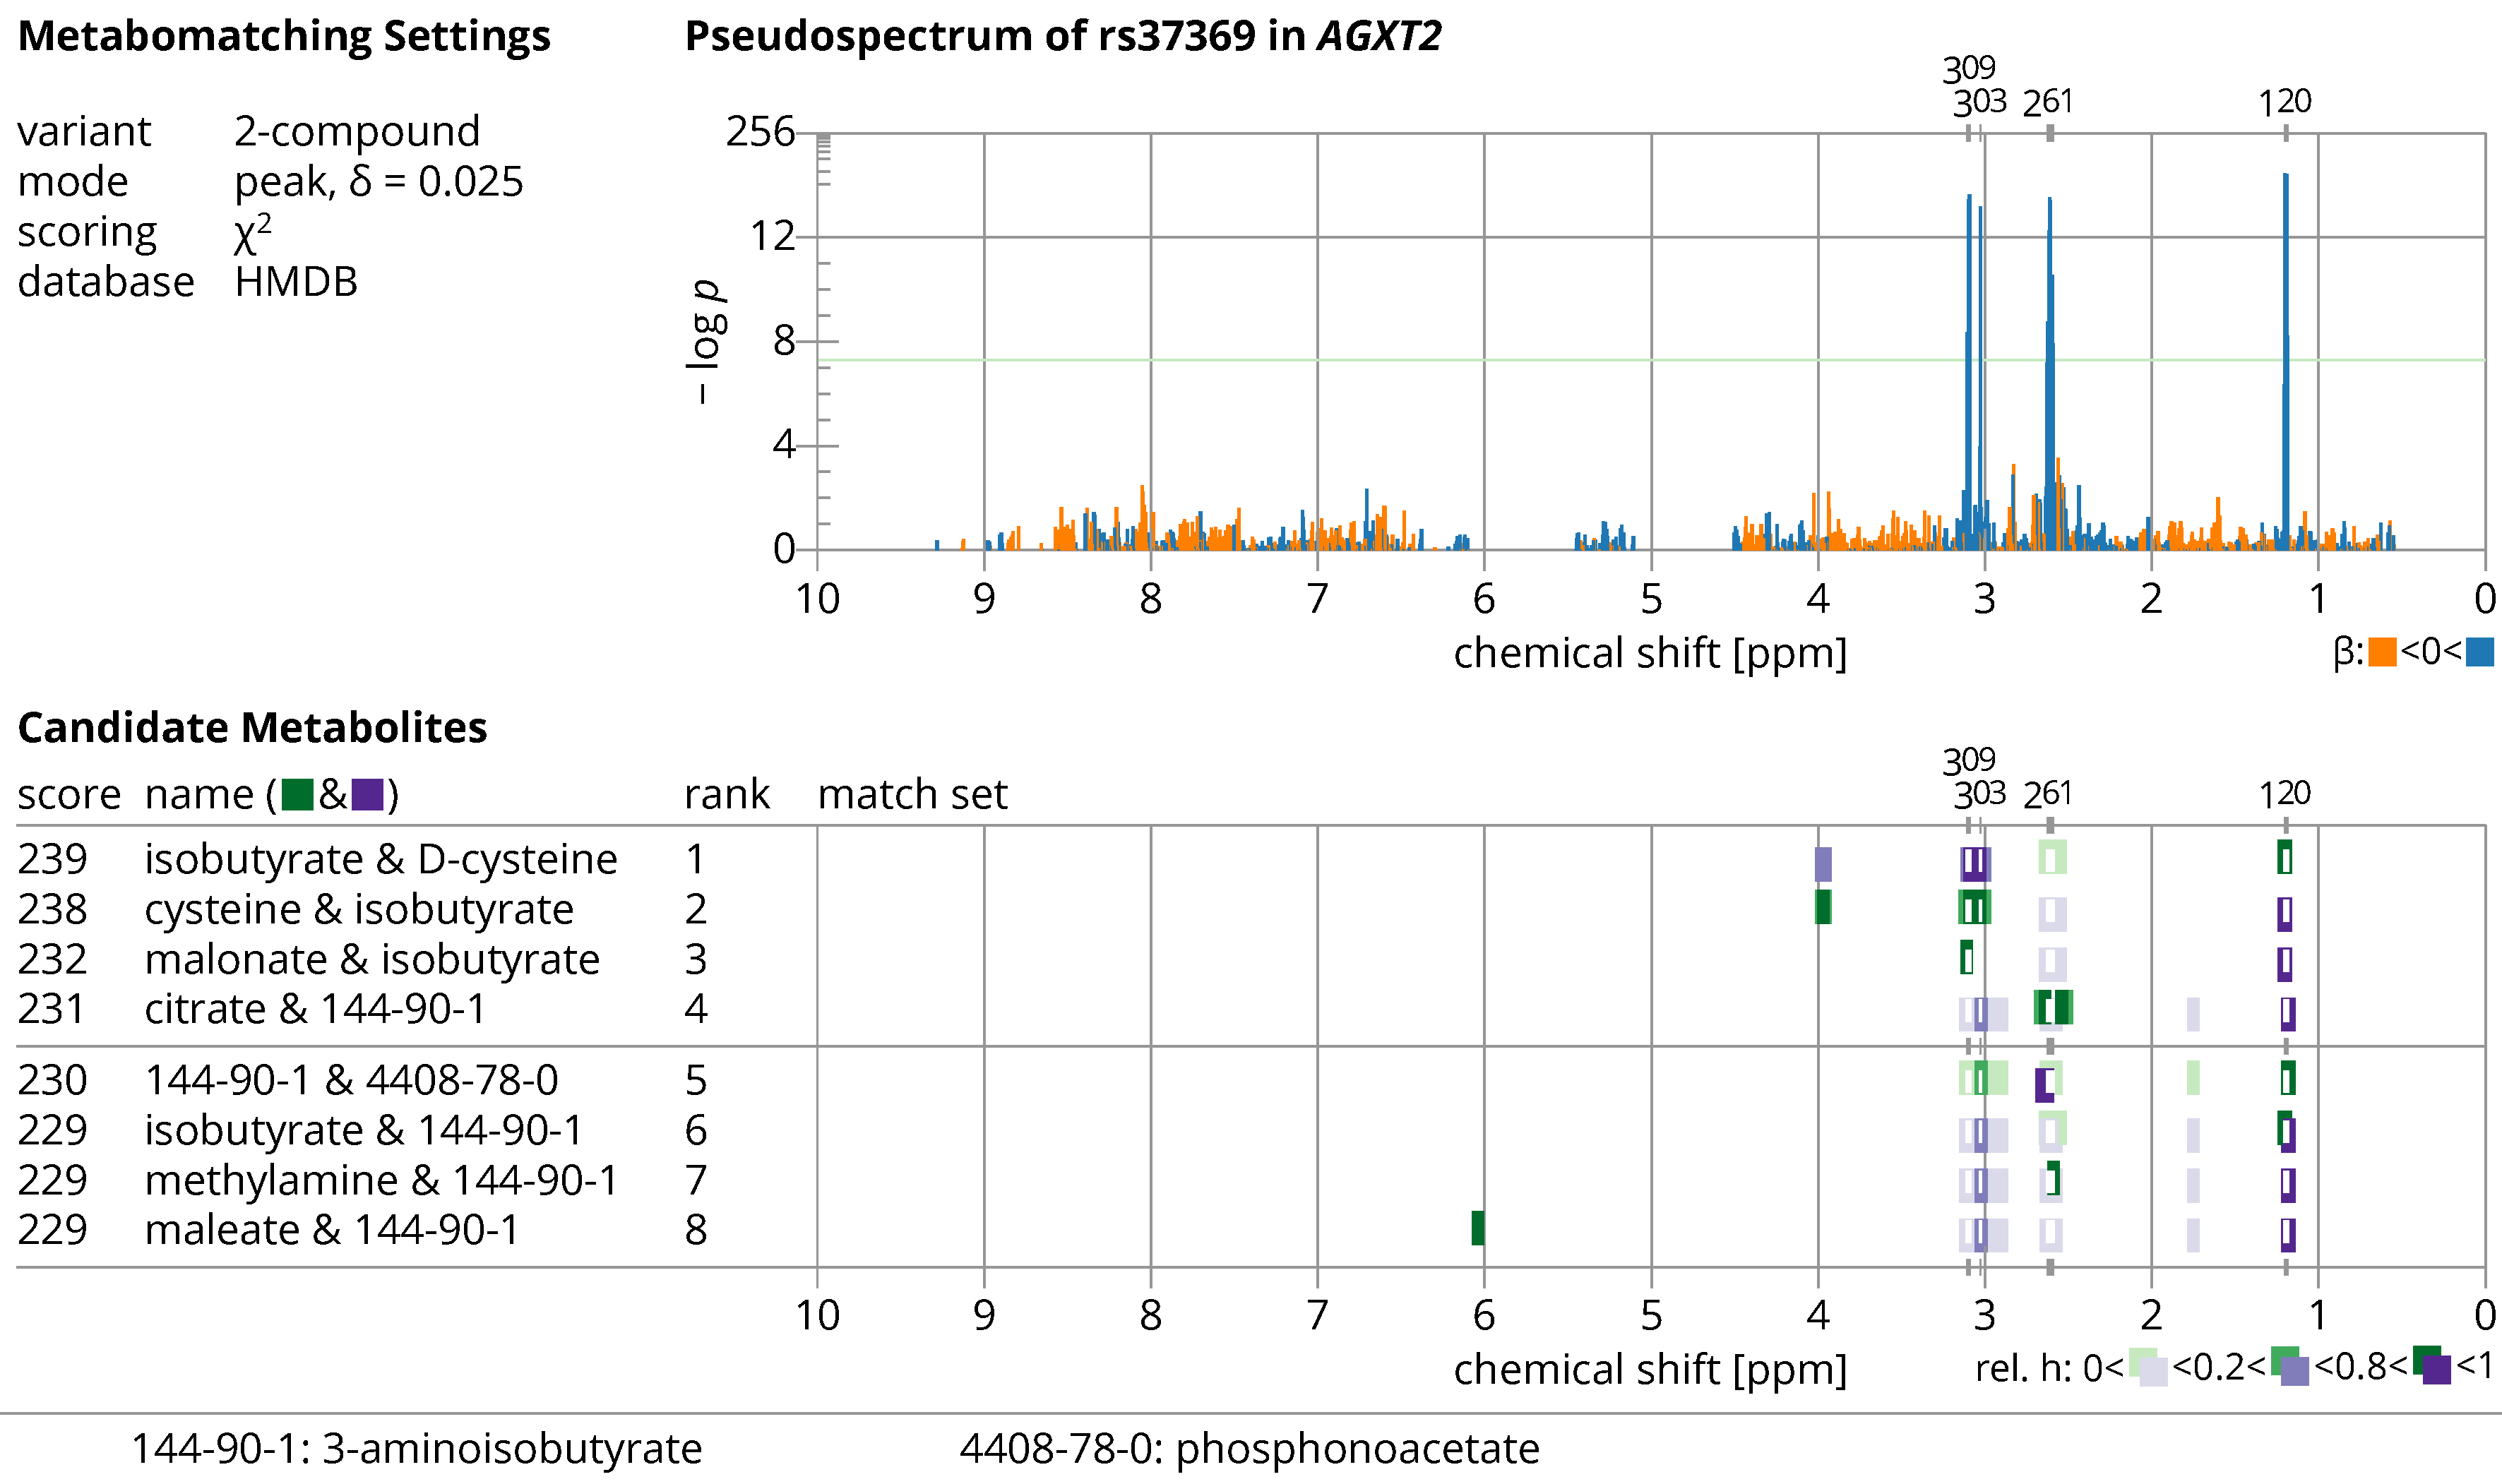
\includegraphics[width=18cm]{f2.pdf}
\caption{2-compound metabomatching results. When running 2-compound metabomatching, pairs of candidate metabolites are scored and ranked. As a result the \emph{Candidate Metabolites} panel lists the names and spectra of two metabolites, with the spectra colored green for one metabolite, and purple for the other. Where metabolite names would overrun the \emph{name} column, CASRN are listed instead, and a CASRN to name table is printed at the bottom of the figure. \label{fig:2}}
\end{figure}
\end{document}

